\begin{figure}[htbp]
\centering 
  \subfloat[Parameter space plot, $AoR_{exp} = 38.85 ^\circ$.]{
	  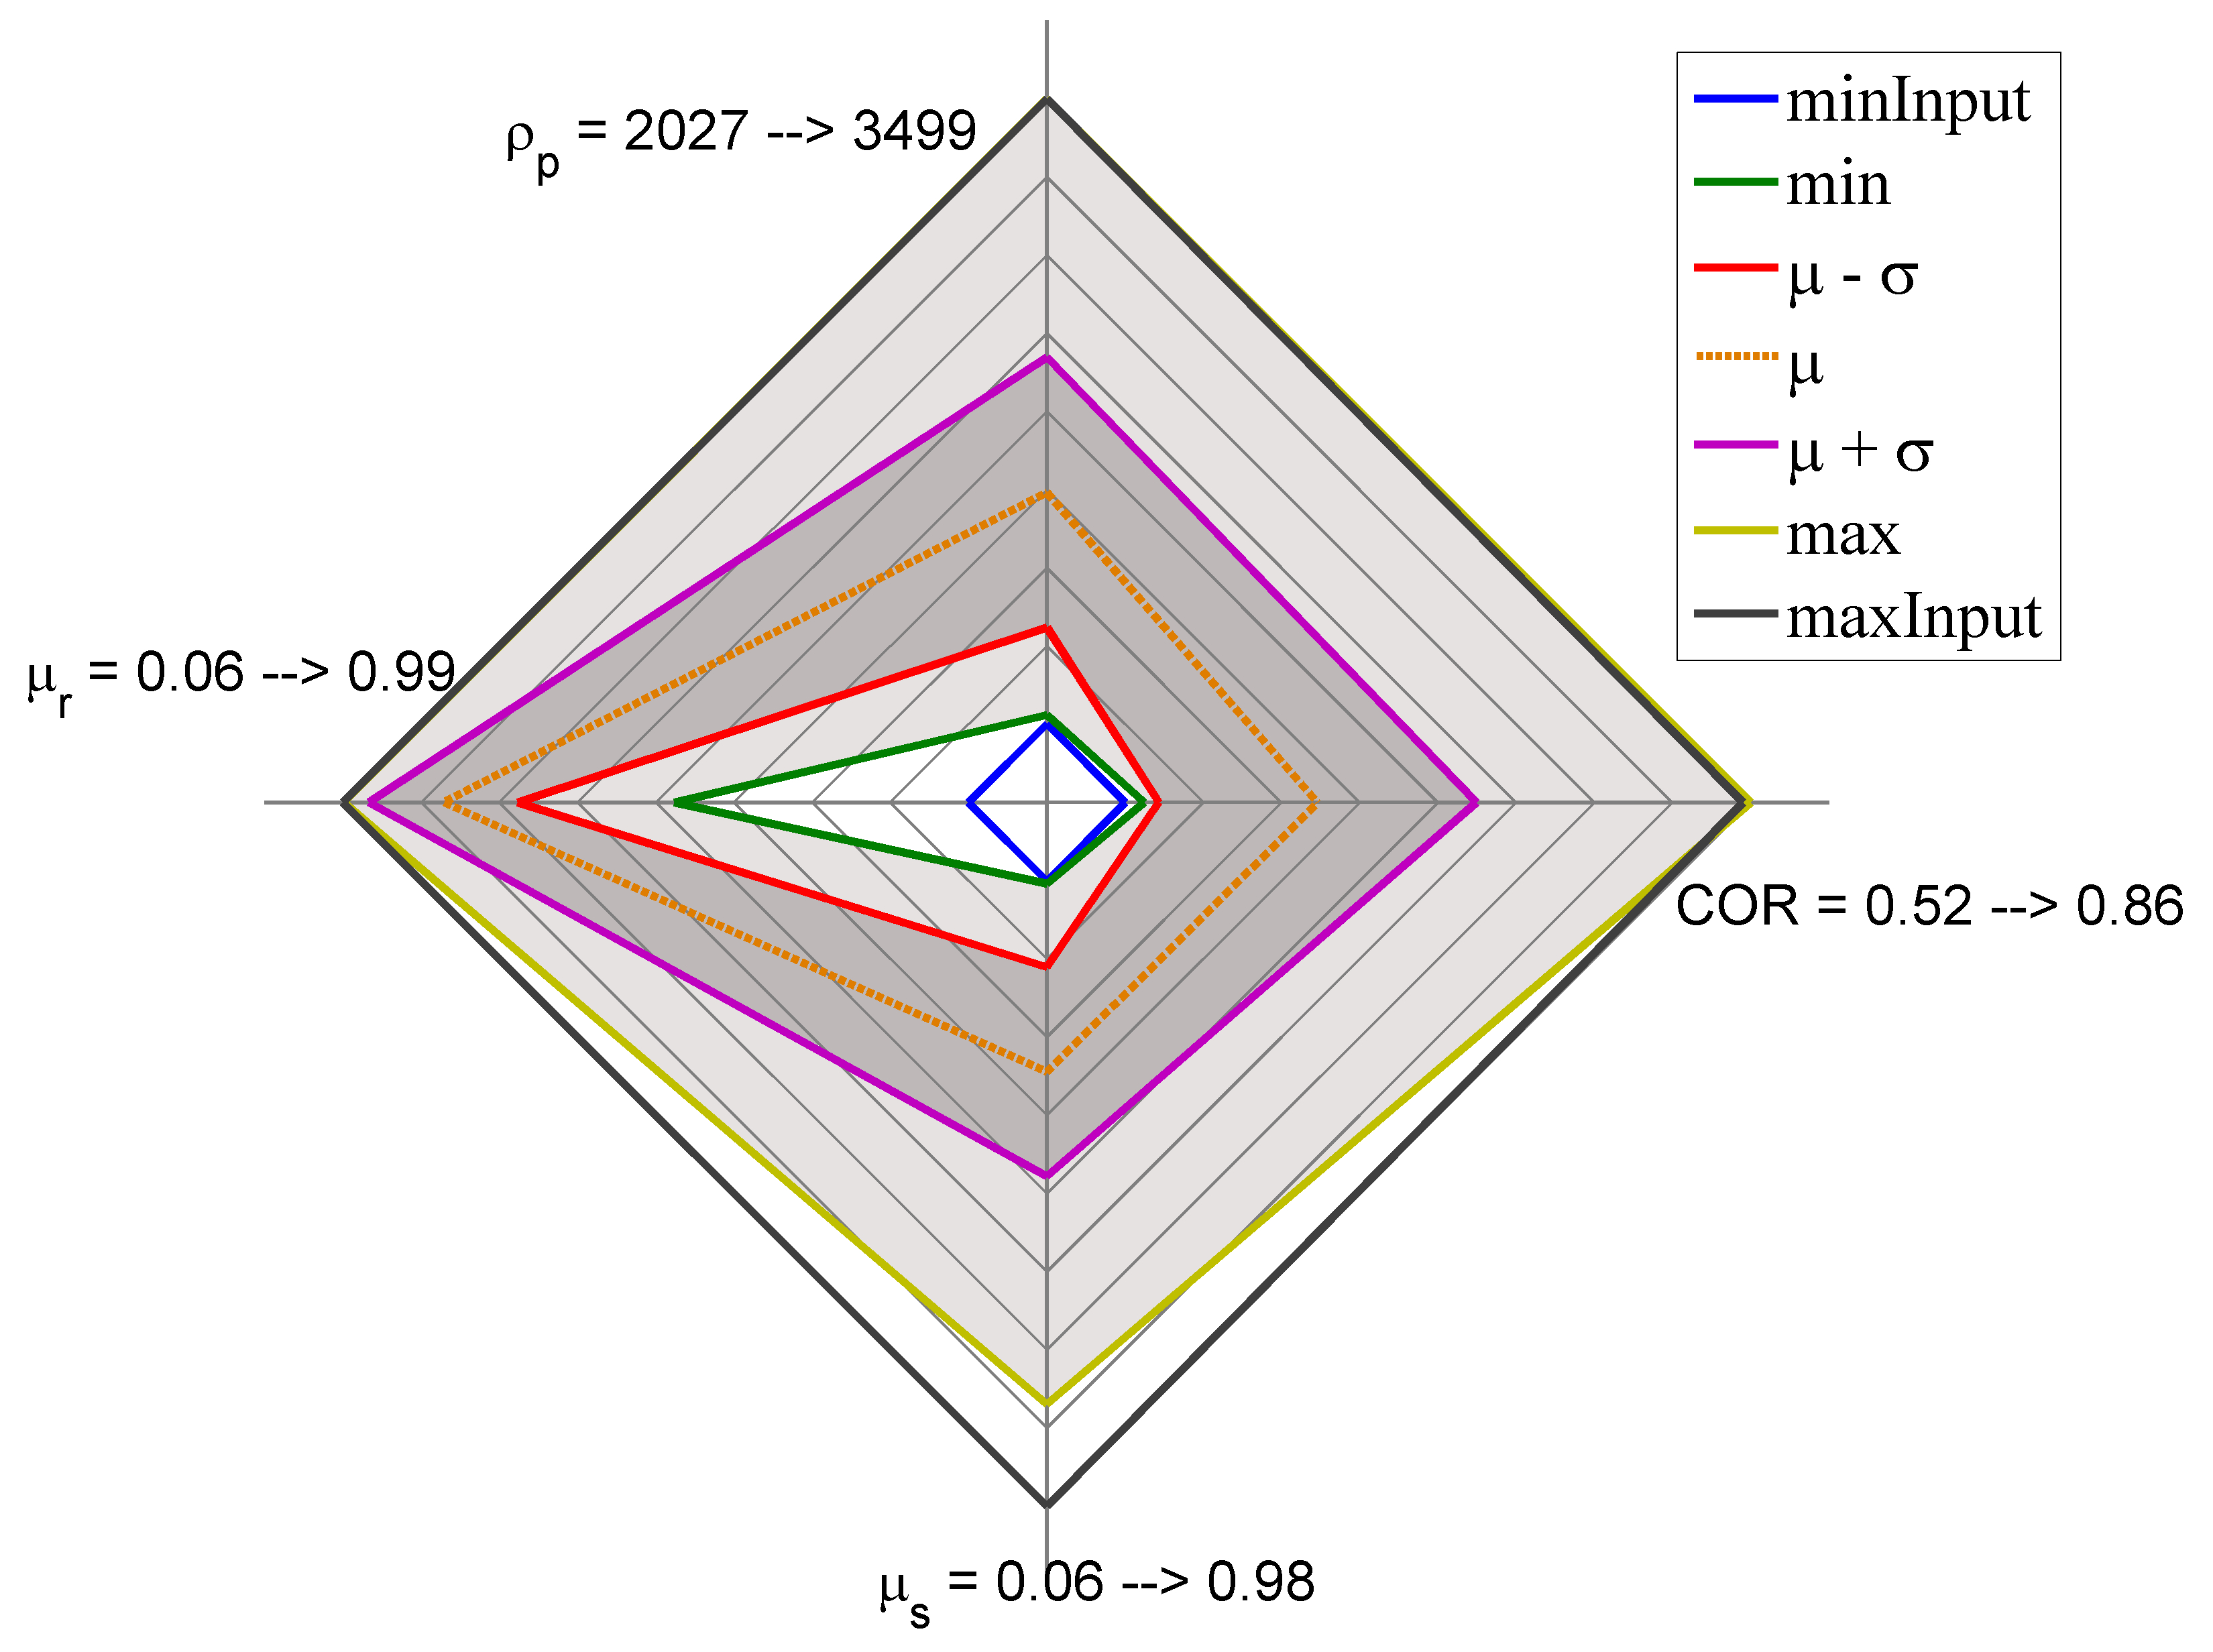
\includegraphics[width=.40\columnwidth]{images/031radarpirker1aor}
	  \label{fig:031radarpirker1aor}
  }
  \quad
    \subfloat[Box plot, $AoR_{exp} = 38.85 ^\circ$.]{
	  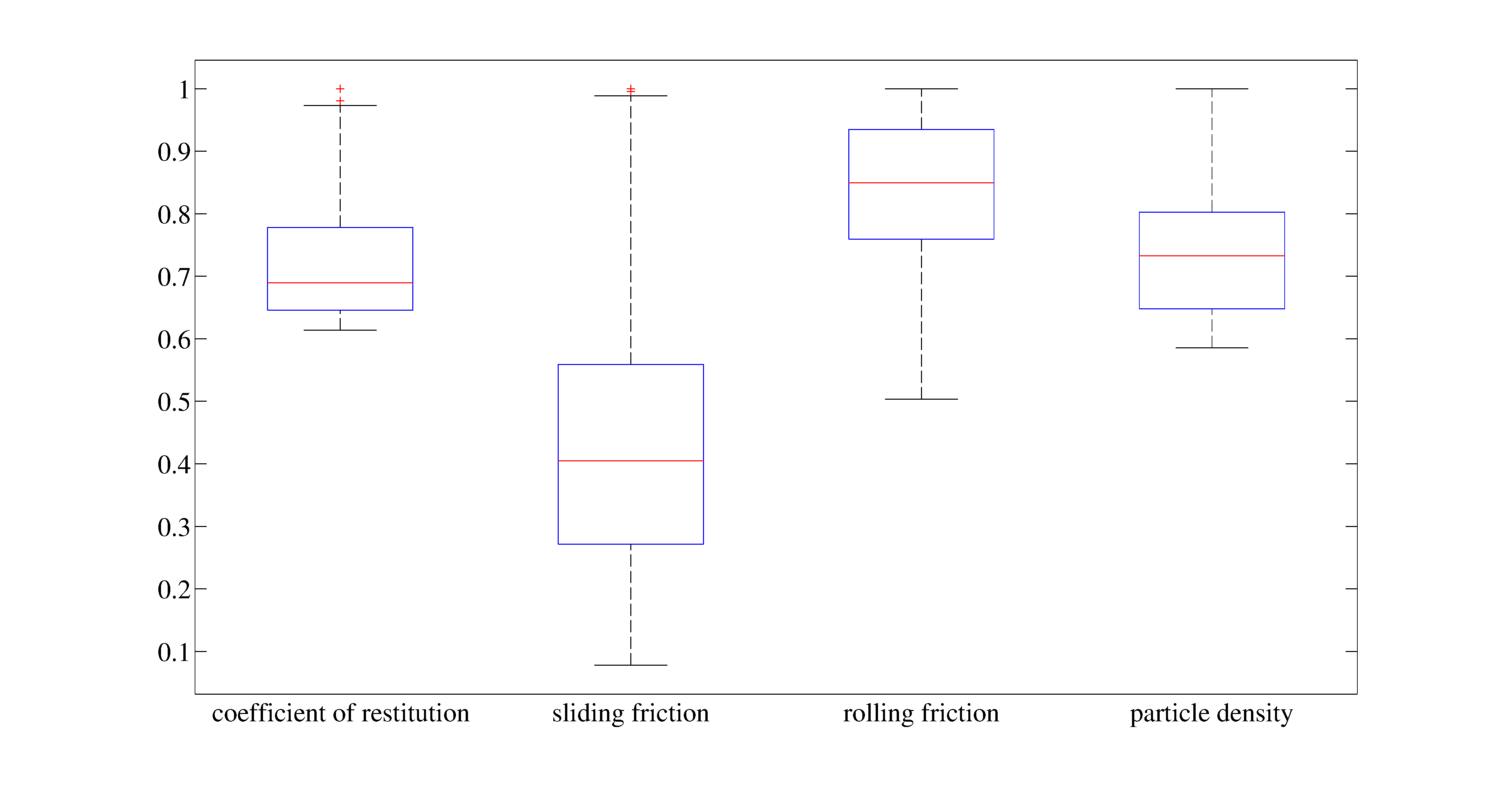
\includegraphics[width=.40\columnwidth]{images/076aorboxplot}
	  \label{fig:076aorboxplot}
  }
  \\
  \subfloat[Parameter space plot, $AoR_{exp} = 38.85 
        ^\circ$ \& $SSC$: $\sigma_n=10070$ Pa.]{
	  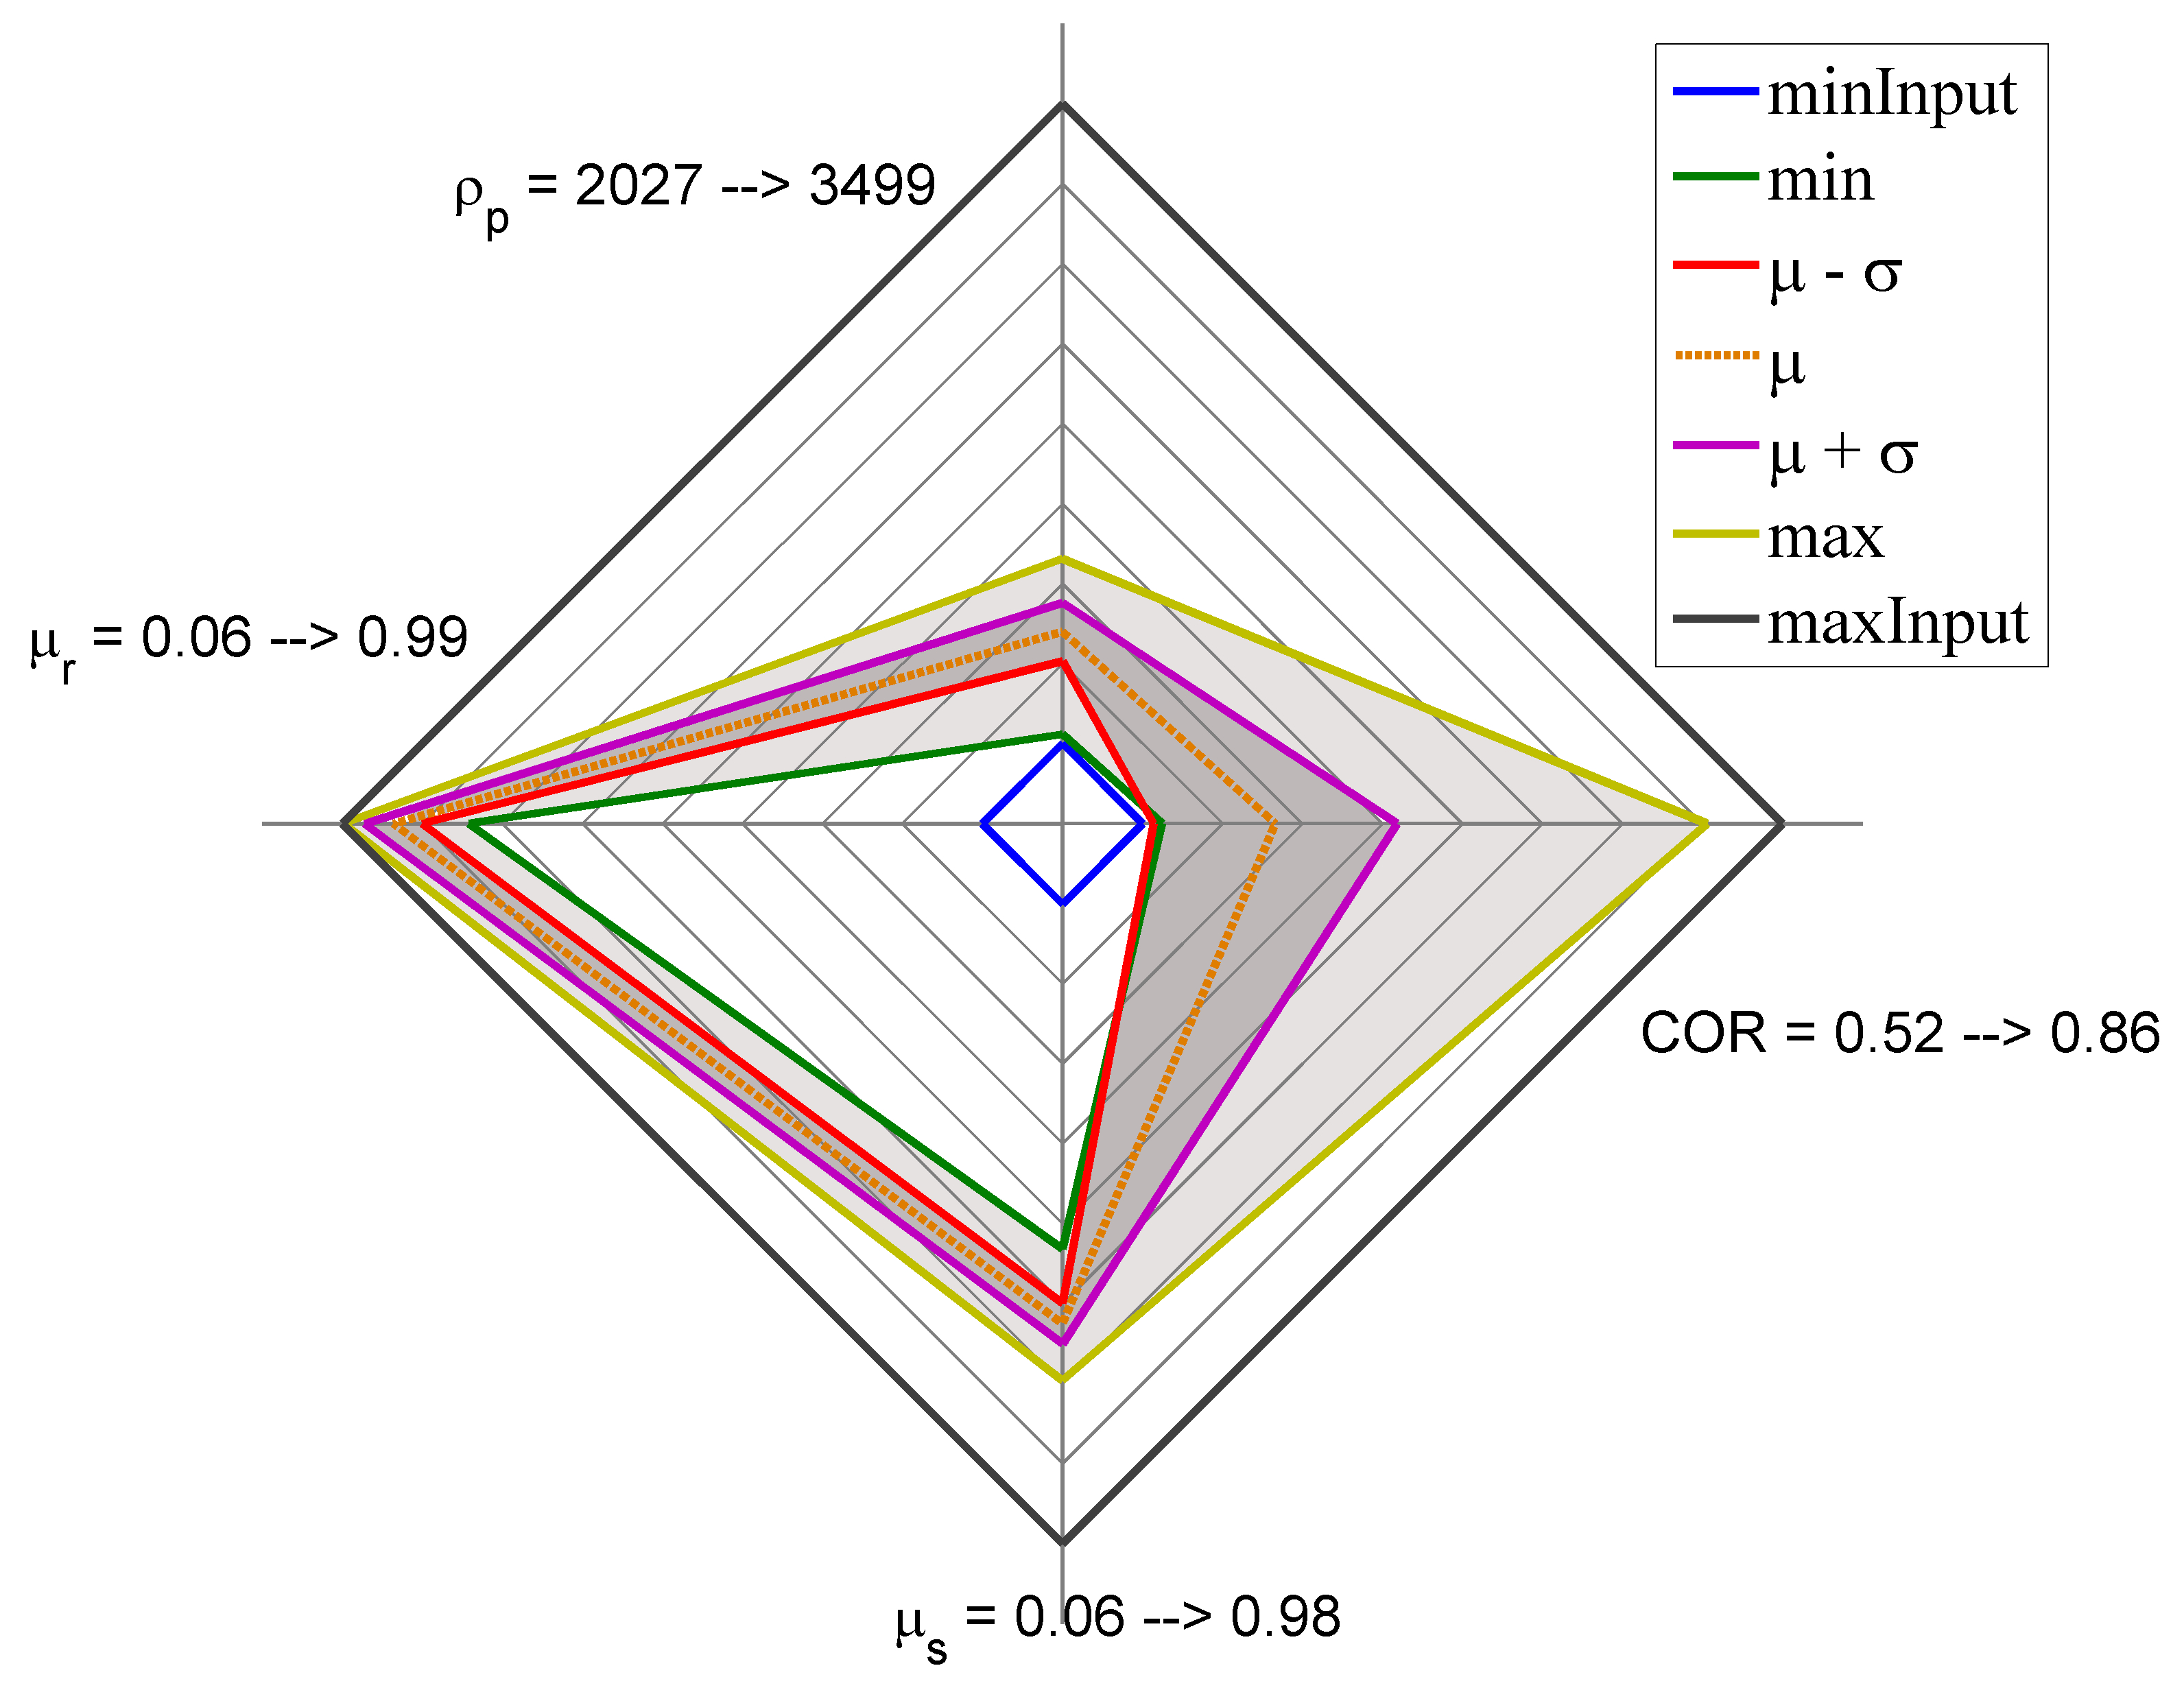
\includegraphics[width=.40\columnwidth]{images/033radarpirker1schulze10070aor}
	  \label{fig:033radarpirker1schulze10070aor}
  }
  \quad
    \subfloat[Box plot, $AoR_{exp} = 38.85
        ^\circ$ \& $SSC$: $\sigma_n=10070$ Pa.]{
	  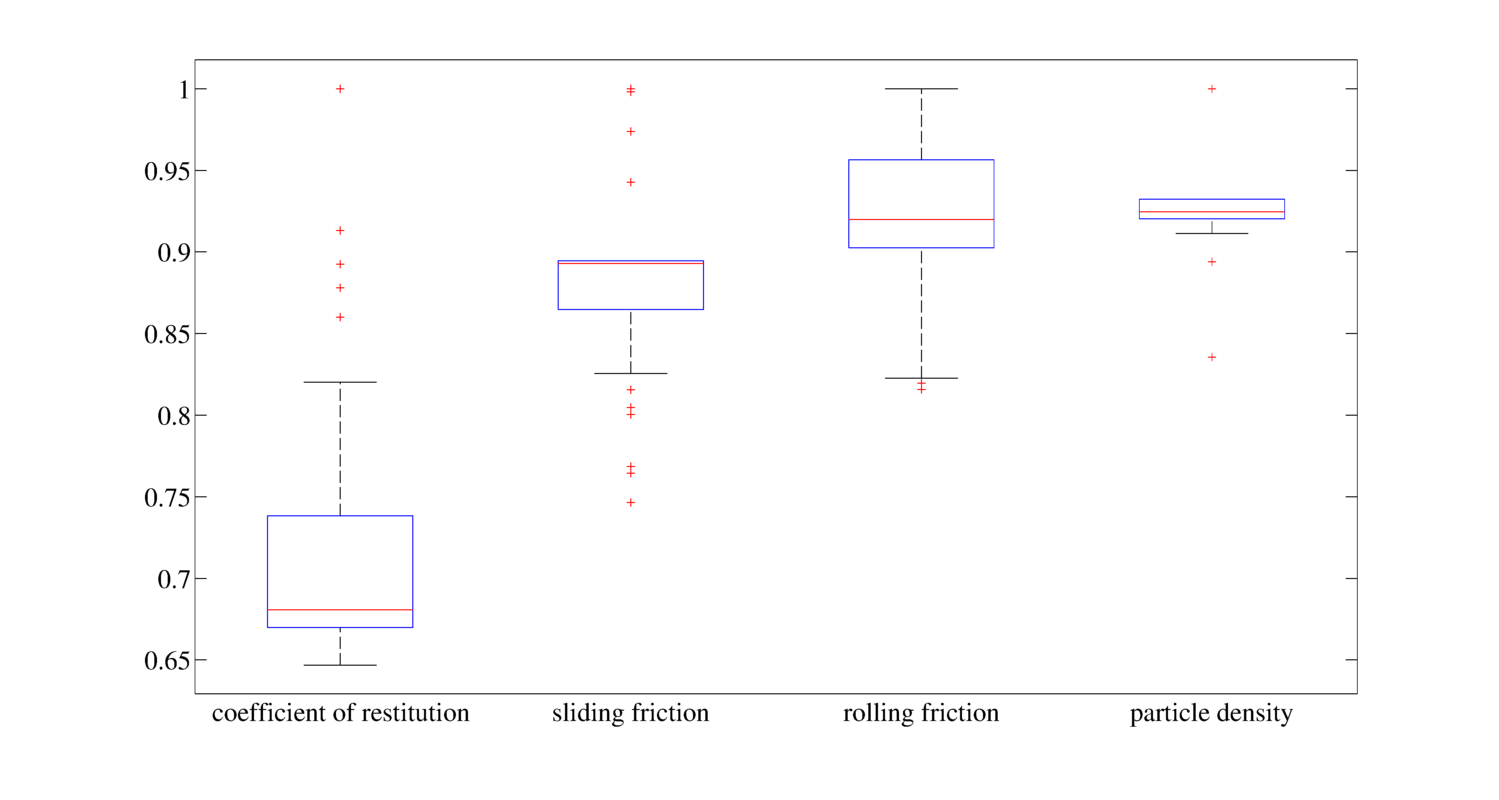
\includegraphics[width=.40\columnwidth]{images/078mergeboxplot}
	  \label{fig:078mergeboxplot}  }
  \\
  \caption{AoR and merge parameter space plots.}
  \label{fig:081aorandmergeparameterspaceplots}
\end{figure}